\chapter{Desarrollo Experimental}

\section{Experimento 1: Contrastación de Voltímetro Analógico}
Se montó un esquema en paralelo entre la fuente, el multímetro analógico UNIVO y el patrón digital Pro'sKit MT-1210. 

\begin{figure}[!ht]
    \centering
    \begin{circuitikz}[american, scale=1.1]
    % Fuente Vcc
    \draw (0, 0) rectangle (2, 2) node[midway] {\Large Vcc};
    
    % Línea superior
    \draw (2, 1.6) -- (8.5, 1.6);
    
    % Línea inferior
    \draw (2, 0.4) -- (8.5, 0.4);
    
    % Instrumento Patrón
    \draw (4, 1.6) to[voltmeter, *-*] (4, 0.4);
    \node[anchor=west, align=left, xshift=0.6cm] at (4, 1) {Instrumento\\Patrón};
    
    % Instrumento Contrastado
    \draw (8.5, 1.6) to[voltmeter, *-*] (8.5, 0.4);
    \node[anchor=west, align=left, xshift=0.6cm] at (8.5, 1) {Instrumento\\Contrastado};
    
\end{circuitikz}

    \caption{Esquema para contrastación del voltímetro analógico.}
    \label{fig:esquema_contrastacion}
\end{figure}

Se procedió a variar la tensión de la fuente, alineando la aguja del UNIVO exactamente sobre las divisiones de la escala
($V_L$), y tomando la lectura del patrón digital ($V_P$). Se efectuó una pasada ascendente y una descendente para
contemplar histéresis y rozamiento mecánico del galvanómetro. En el cuadro \ref{tab:contrastacion} se presentan los
valores registrados durante el ensayo.

\begin{figure}[!ht]
    \centering
    \begin{subfigure}[t]{0.45\textwidth}
        \centering
        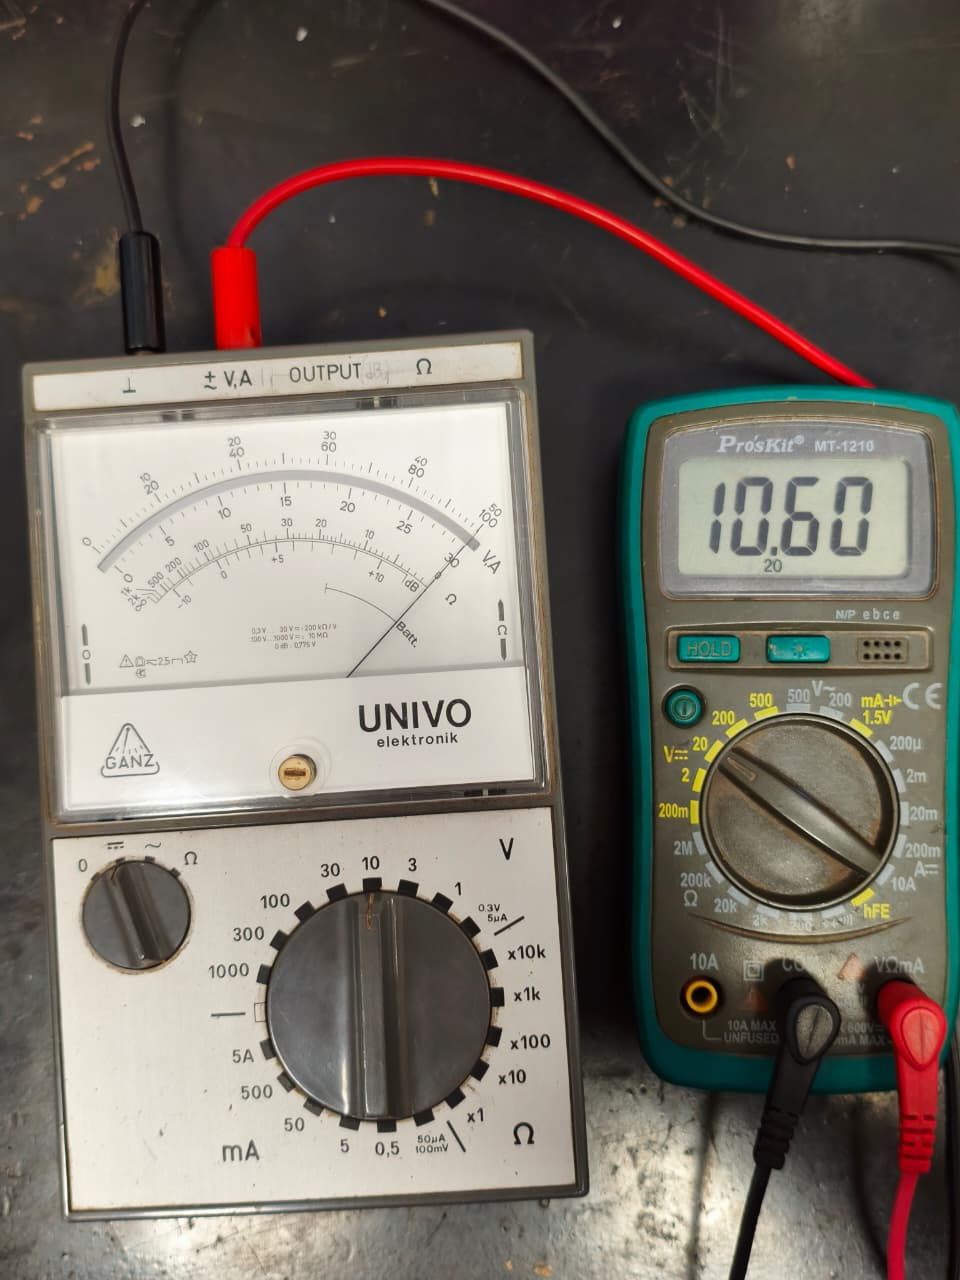
\includegraphics[width=\textwidth]{pictures/Constrastacion_voltimetro_analogico.jpeg}
        \caption{Montaje de contrastación en paralelo.}
    \end{subfigure}
    \hfill
    \begin{subfigure}[t]{0.45\textwidth}
        \centering
        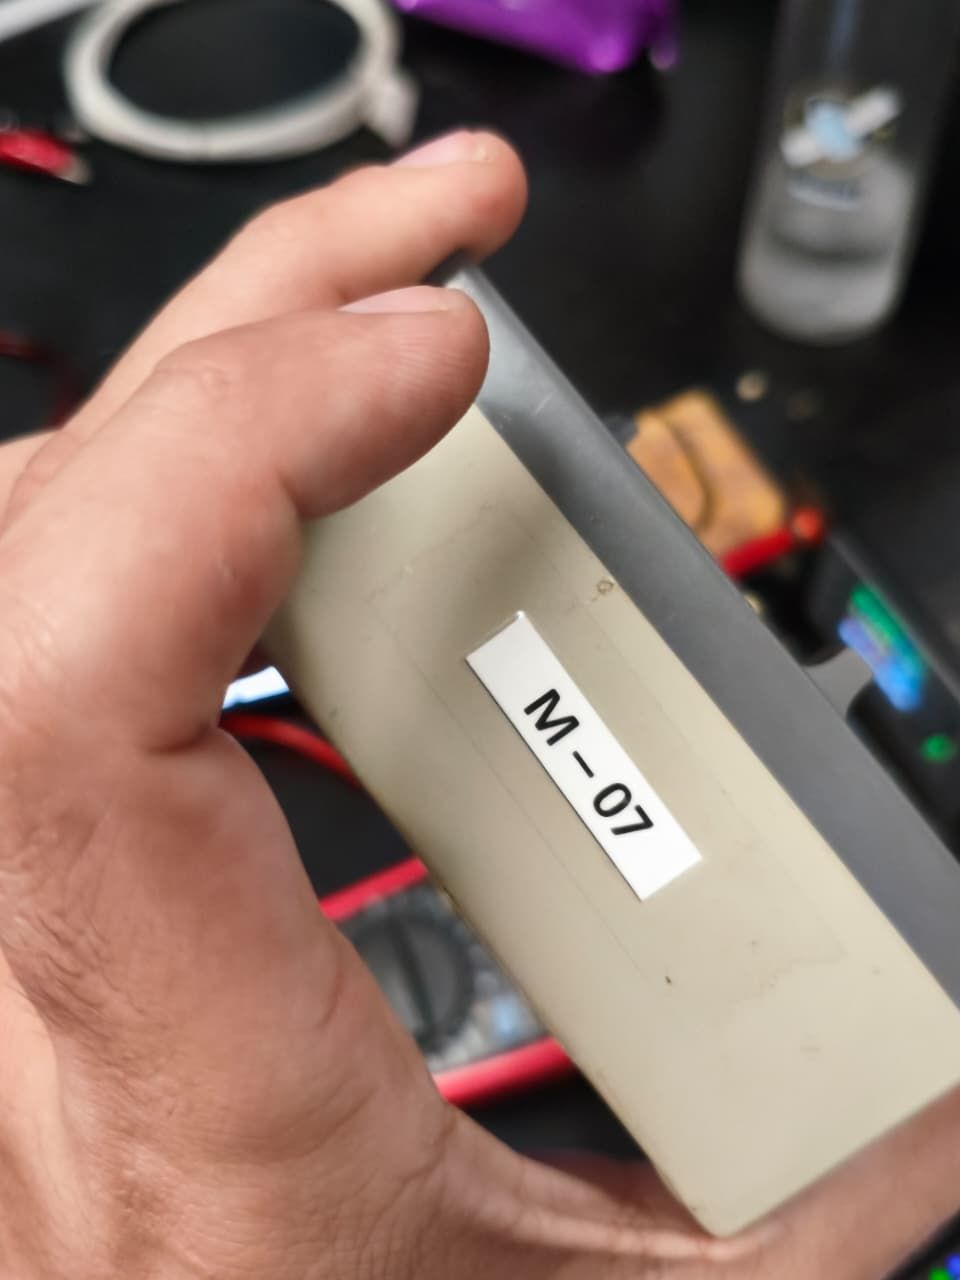
\includegraphics[width=\textwidth]{pictures/Comprobacion_serialnumber_volt_analogico.jpeg}
        \caption{Identificación del instrumento bajo prueba.}
    \end{subfigure}
    \caption{Proceso de contrastación del multímetro analógico UNIVO.}
\end{figure}

\begin{table}[!ht]
    \centering
    \resizebox{\textwidth}{!}{
    \begin{tabular}{|c|c|c|c|c|c|c|c|c|c|c|}
        \hline
        $V_L$ [$\V$] & 1 & 2 & 3 & 4 & 5 & 6 & 7 & 8 & 9 & 10 \\ \hline
        $V_P$ (hacia arriba) & 1,01 & 2,14 & 3,20 & 4,25 & 5,32 & 6,39 & 7,46 & 8,52 & 9,59 & 10,60 \\ \hline
        $V_P$ (hacia abajo) & 0,99 & 2,11 & 3,17 & 4,23 & 5,31 & 6,38 & 7,45 & 8,51 & 9,57 & 10,60 \\ \hline
        $\Delta V$ (mayor valor) & 0,01 & 0,14 & 0,20 & 0,25 & 0,32 & 0,39 & 0,46 & 0,52 & 0,59 & 0,60 \\ \hline
    \end{tabular}}
    \caption{Valores obtenidos de la contrastación. $V_L$: indicado, $V_P$: patrón, $\Delta V$: Error absoluto.}
    \label{tab:contrastacion}
\end{table}

\subsection{Curva de Contrastación}
\begin{figure}[!ht]
    \centering
    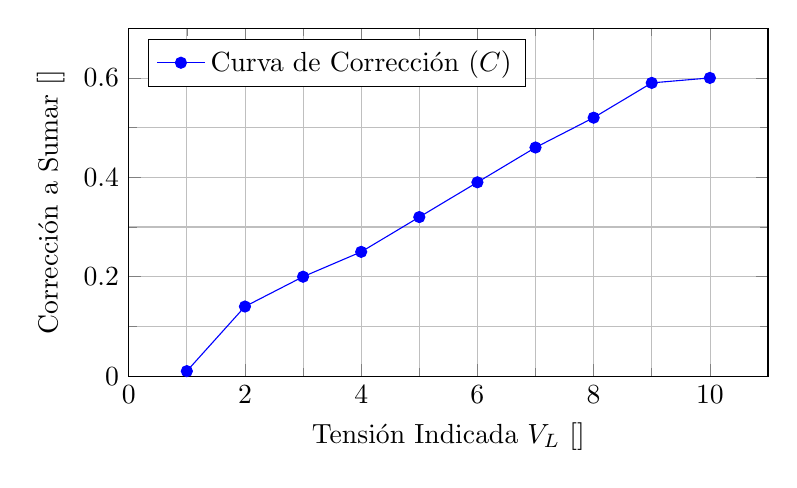
\begin{tikzpicture}
    \begin{axis}[
        width=0.8\textwidth,
        height=6cm,
        xlabel={Tensión Indicada $V_L$ [$\V$]},
        ylabel={Corrección a Sumar [$\V$]},
        xmin=0, xmax=11,
        ymin=0, ymax=0.7,
        grid=both,
        minor tick num=1,
        major grid style={line width=.2pt,draw=gray!50},
        legend pos=north west
    ]
    \addplot[color=blue, mark=*] coordinates {
        (1, 0.01)
        (2, 0.14)
        (3, 0.20)
        (4, 0.25)
        (5, 0.32)
        (6, 0.39)
        (7, 0.46)
        (8, 0.52)
        (9, 0.59)
        (10, 0.60)
    };
    \legend{Curva de Corrección ($C$)}
    \end{axis}
\end{tikzpicture}

    \caption{Curva de contrastación: Valores a sumar al instrumento bajo prueba en función de su indicación.}
    \label{fig:curva_contrastacion}
\end{figure}

\vspace{0.5cm}
\begin{figure}[!ht]
    \centering
    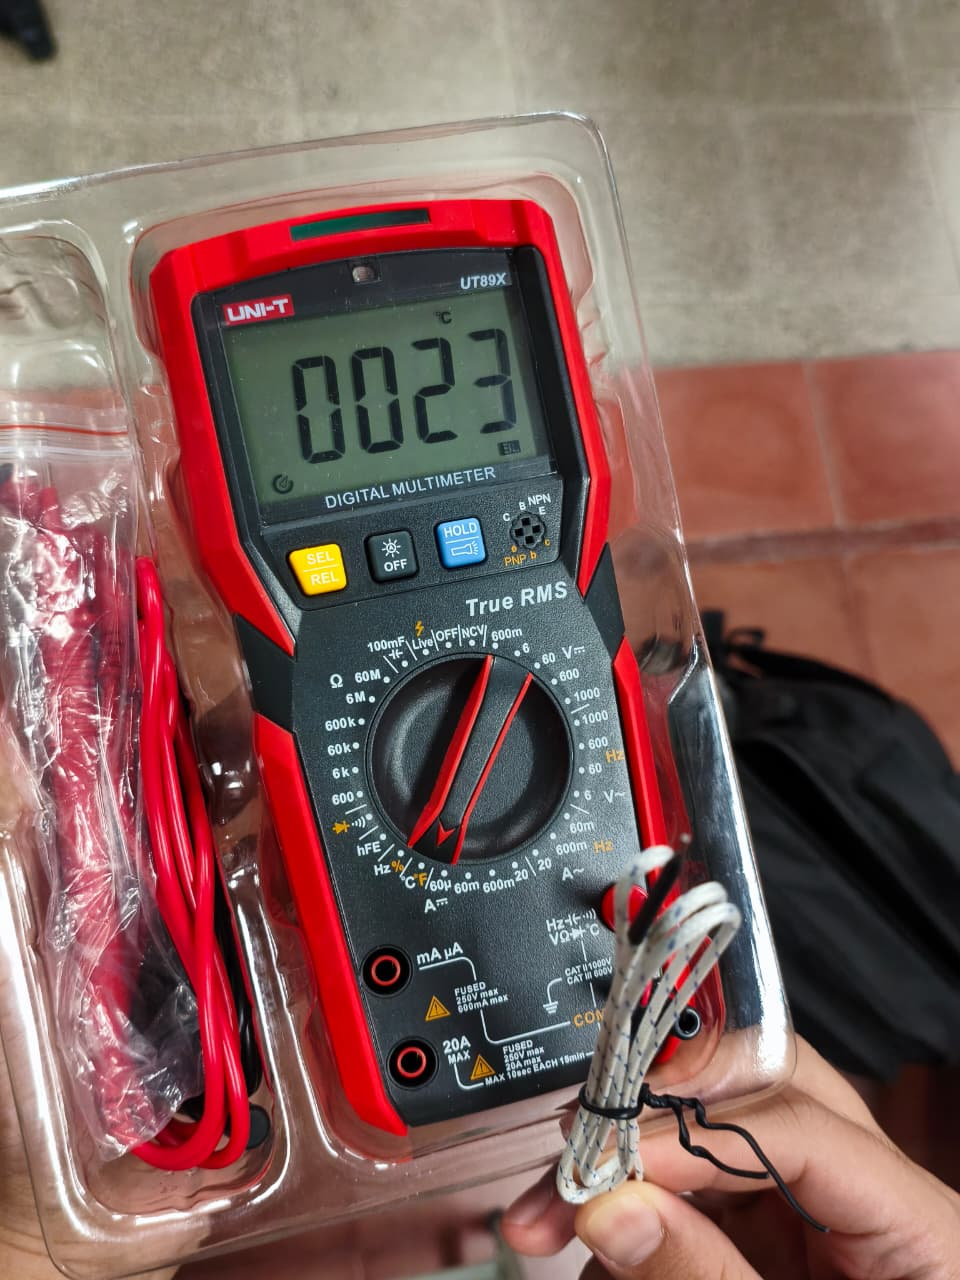
\includegraphics[width=0.4\textwidth]{pictures/Temperatura_ambiente.jpeg}
    \caption{Medición de la temperatura ambiente durante la experiencia.}
    \label{fig:temp_ambiente}
\end{figure}

En el cuadro \ref{tab:trazabilidad} se detallan las condiciones de trazabilidad, instrumental utilizado y parámetros ambientales registrados durante la experiencia.

\begin{table}[!ht]
    \centering
    \begin{tabular}{|p{4cm}|p{4cm}|p{3cm}|p{3cm}|}
        \hline
        \textbf{Inst. Contrastado} & \textbf{Patrón} & \textbf{Fecha y Hora} & \textbf{Operador} \\ \hline
        Marca: UNIVO \newline Nro: M-07 & Marca: Pro'sKit \newline Nro: S/D & 09/04/2026 17:48 hs & Franco Palombo \\ \hline
        \multicolumn{4}{|l|}{\textbf{Temperatura Ambiente:} $23 \Celsius$} \\ \hline
    \end{tabular}
    \caption{Datos de trazabilidad de la contrastación.}
    \label{tab:trazabilidad}
\end{table}

\subsection{Cálculo del Índice de Clase}
A partir de los datos consignados en el cuadro \ref{tab:contrastacion}, se identifica el Error Absoluto Máximo ($\Delta V = 0,60 \V$ en $V_L = 10 \V$) y se
calcula el índice de clase:
\begin{equation}
    Clase = \frac{0,60}{10} \cdot 100 = 6 \percent
    \label{eq:clase}
\end{equation}
\textit{(Redondear hacia arriba el resultado). Comprobación: El fabricante del UNIVO declara una Clase de $2,5 \percent$.
¿Guarda coherencia el valor obtenido?} \textbf{El valor obtenido no guarda coherencia con lo declarado por el
fabricante. El instrumento presenta un índice de clase experimental del $6 \percent$, lo que significa que se encuentra
fuera de especificación y requeriría una recalibración o reparación, ya que su error supera ampliamente el límite de
$2,5 \percent$ del fondo de escala establecido para su correcto funcionamiento.}

\section{Experimento 2: Medición de Resistencia por 4 Terminales}
Para medir resistencias de valores muy bajos (inferiores a unos pocos Ohms), el método convencional de dos puntas introduce
un error inadmisible debido a que la resistencia de los cables y de contacto se suma directamente al valor de la probeta.
Para eliminar este efecto, se implementó el \textbf{método de 4 terminales (Kelvin)}, cuyo principio circuital se presenta
en la figura \ref{fig:esquema_4terminales}.

\begin{figure}[!ht]
    \centering
    \begin{circuitikz}[american, scale=1.05]
    % Generador de corriente constante (Fuente SK150)
    \draw (0, 0.5) rectangle (2.6, 3.5) node[midway, align=center] {\textbf{Fuente}\\\textbf{SK150}\\($I_{\text{cte}}$)};
    
    % Rama superior de corriente con miliamperímetro
    \draw (2.6, 3.0) -- (3.2, 3.0) to[ammeter, l={\small UT33A+ ($I$)}] (5.2, 3.0) 
          to[R, l={\small $r_{c1}$}, *-] (7.2, 3.0) -- (8.2, 3.0) -- (8.2, 2.6);
    
    % Rama inferior de retorno de corriente
    \draw (2.6, 1.0) -- (5.2, 1.0) 
          to[R, l_={\small $r_{c2}$}, *-] (7.2, 1.0) -- (8.2, 1.0) -- (8.2, 1.4);
    
    % Probeta bajo prueba Rx
    \draw (8.2, 2.6) to[R, l_={\textbf{$R_x$}}, *-*] (8.2, 1.4);
    \node[anchor=west, align=left, font=\scriptsize] at (8.35, 2.0) {\textbf{Probeta}\\(cable 12 m)};
    
    % Terminales Kelvin (1, 2, 3, 4)
    \node[circle, fill=blue!20, draw=blue, inner sep=1.5pt, font=\scriptsize\bfseries] at (8.2, 3.0) {1};
    \node[circle, fill=blue!20, draw=blue, inner sep=1.5pt, font=\scriptsize\bfseries] at (8.2, 1.0) {2};
    \node[circle, fill=red!20, draw=red, inner sep=1.5pt, font=\scriptsize\bfseries] at (8.2, 2.6) {3};
    \node[circle, fill=red!20, draw=red, inner sep=1.5pt, font=\scriptsize\bfseries] at (8.2, 1.4) {4};
    
    % Puntas de sensado de potencial (interiores)
    \draw (8.2, 2.6) -- (9.2, 2.6) to[R, l={\small $r_{c3}$}] (11.0, 2.6) -- (11.8, 2.6) -- (11.8, 2.4);
    \draw (8.2, 1.4) -- (9.2, 1.4) to[R, l_={\small $r_{c4}$}] (11.0, 1.4) -- (11.8, 1.4) -- (11.8, 1.6);
    
    % Voltímetro
    \draw (11.8, 2.4) to[voltmeter, l={\small UT33A+ ($V$)}, *-*] (11.8, 1.6);
\end{circuitikz}
    \caption{Esquema del circuito de medición de resistencia por 4 terminales (método de Kelvin).}
    \label{fig:esquema_4terminales}
\end{figure}

El circuito separa físicamente el lazo de inyección de corriente del lazo de sensado de potencial:
\begin{itemize}
    \item \textbf{Lazo de Corriente (Terminales 1 y 2):} Una fuente de corriente constante (módulo SK150) inyecta una corriente continua de prueba $I \approx 100\text{ mA}$ medida con un multímetro digital UNI-T UT33A+ en serie. Las caídas de tensión sobre las resistencias de contacto $r_{c1}$ y $r_{c2}$ quedan fuera del circuito de medición de potencial.
    \item \textbf{Lazo de Potencial (Terminales 3 y 4):} Se conectan dos terminales independientes directamente sobre los extremos de la probeta bajo prueba $R_x$ hacia un segundo multímetro digital UNI-T UT33A+ en función voltímetro. Debido a la elevada impedancia de entrada del instrumento ($R_{in} \approx 10\text{ M}\Omega$), la corriente por las puntas de potencial es prácticamente nula ($I_v \approx 0$). Por ende, la caída de tensión sobre las resistencias parásitas $r_{c3}$ y $r_{c4}$ es despreciable ($\Delta V_{r_{c}} \approx 0$), midiendo directamente la tensión $V_{Rx} = I \cdot R_x$.
\end{itemize}

La probeta ensayada consiste en un arrollamiento no inductivo de cable de cobre con una longitud de $12\text{ m} \pm 12\text{ cm}$. En el cuadro \ref{tab:medicion_4term} se muestran los valores medidos en forma simultánea de corriente y caída de tensión, así como el valor resultante de la resistencia.

\begin{table}[!ht]
    \centering
    \begin{tabular}{|c|c|c|}
        \hline
        $V$ [$\mV$] & $I$ [$\mA$] & $R = V/I$ [$\ohm$] \\ \hline
        106,0 & 100,1 & 1,059 \\ \hline
    \end{tabular}
    \caption{Medición directa de tensión y corriente en la probeta por el método de 4 terminales.}
    \label{tab:medicion_4term}
\end{table}

\begin{figure}[!ht]
    \centering
    \begin{subfigure}[t]{0.45\textwidth}
        \centering
        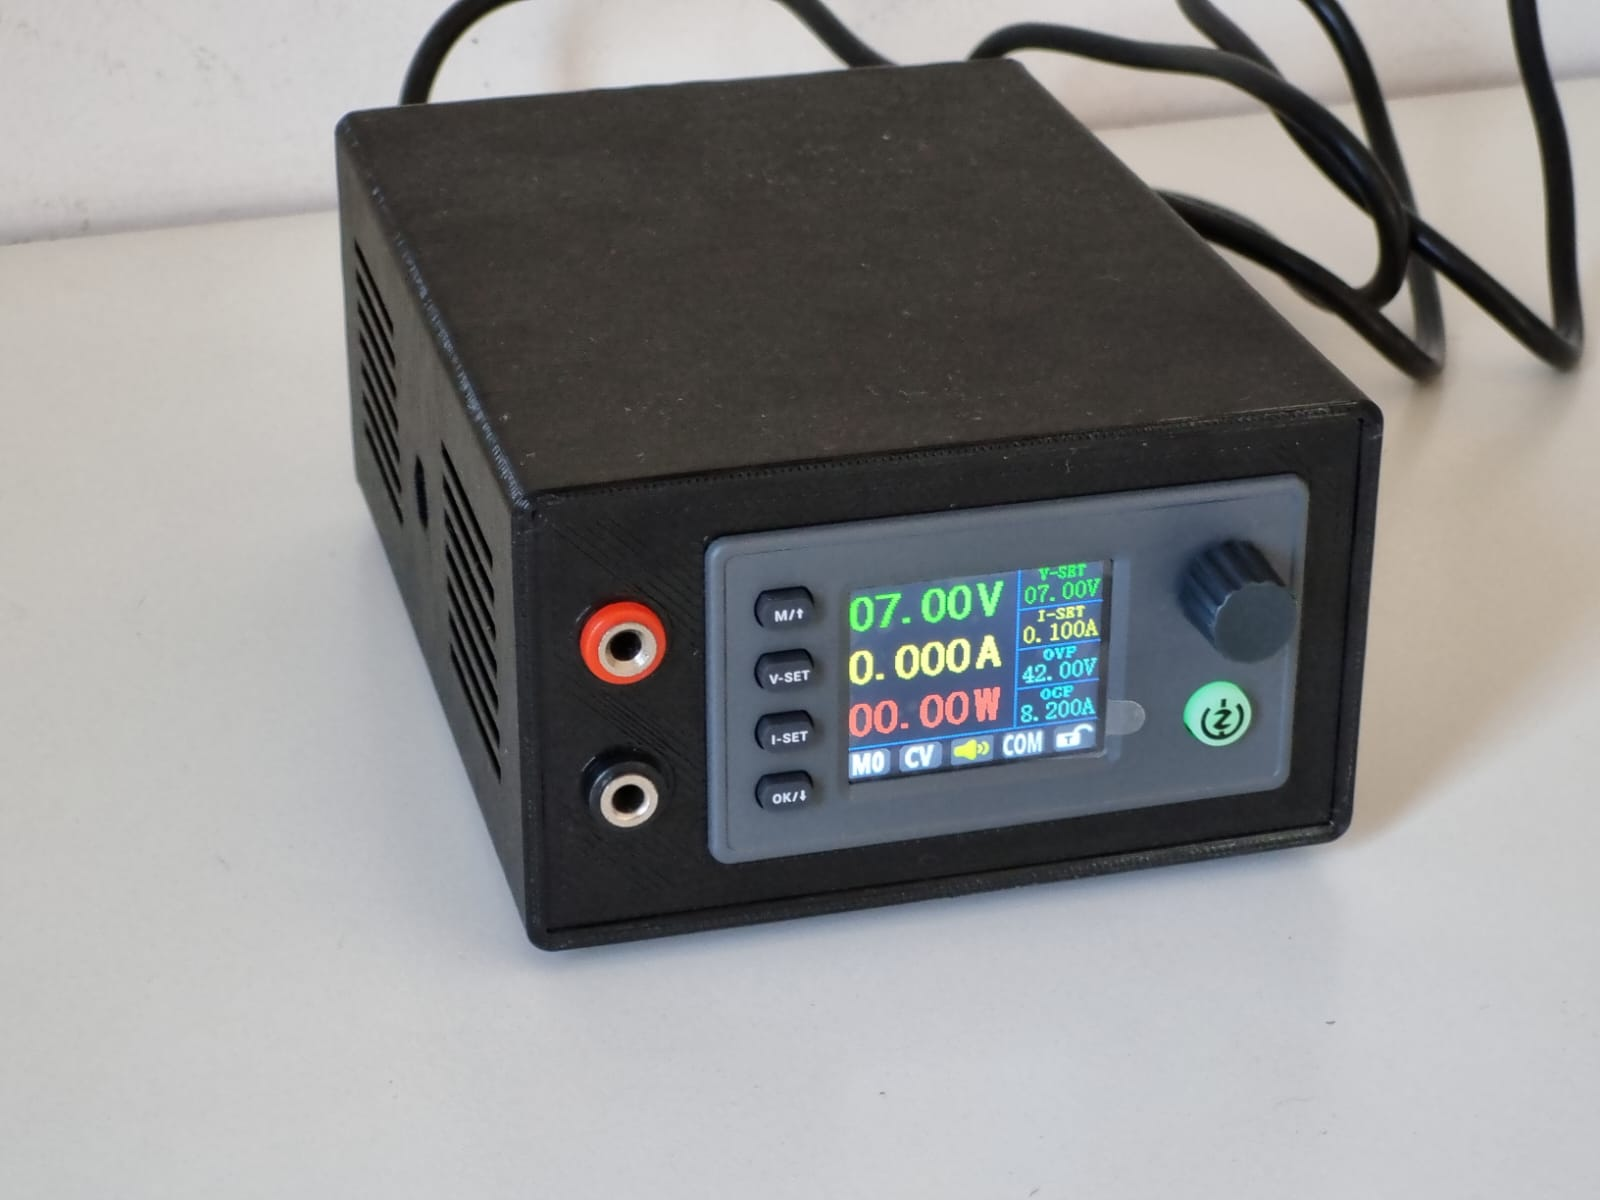
\includegraphics[width=\textwidth]{pictures/Fuente_sk150.jpeg}
        \caption{Fuente de corriente constante SK150.}
    \end{subfigure}
    \hfill
    \begin{subfigure}[t]{0.45\textwidth}
        \centering
        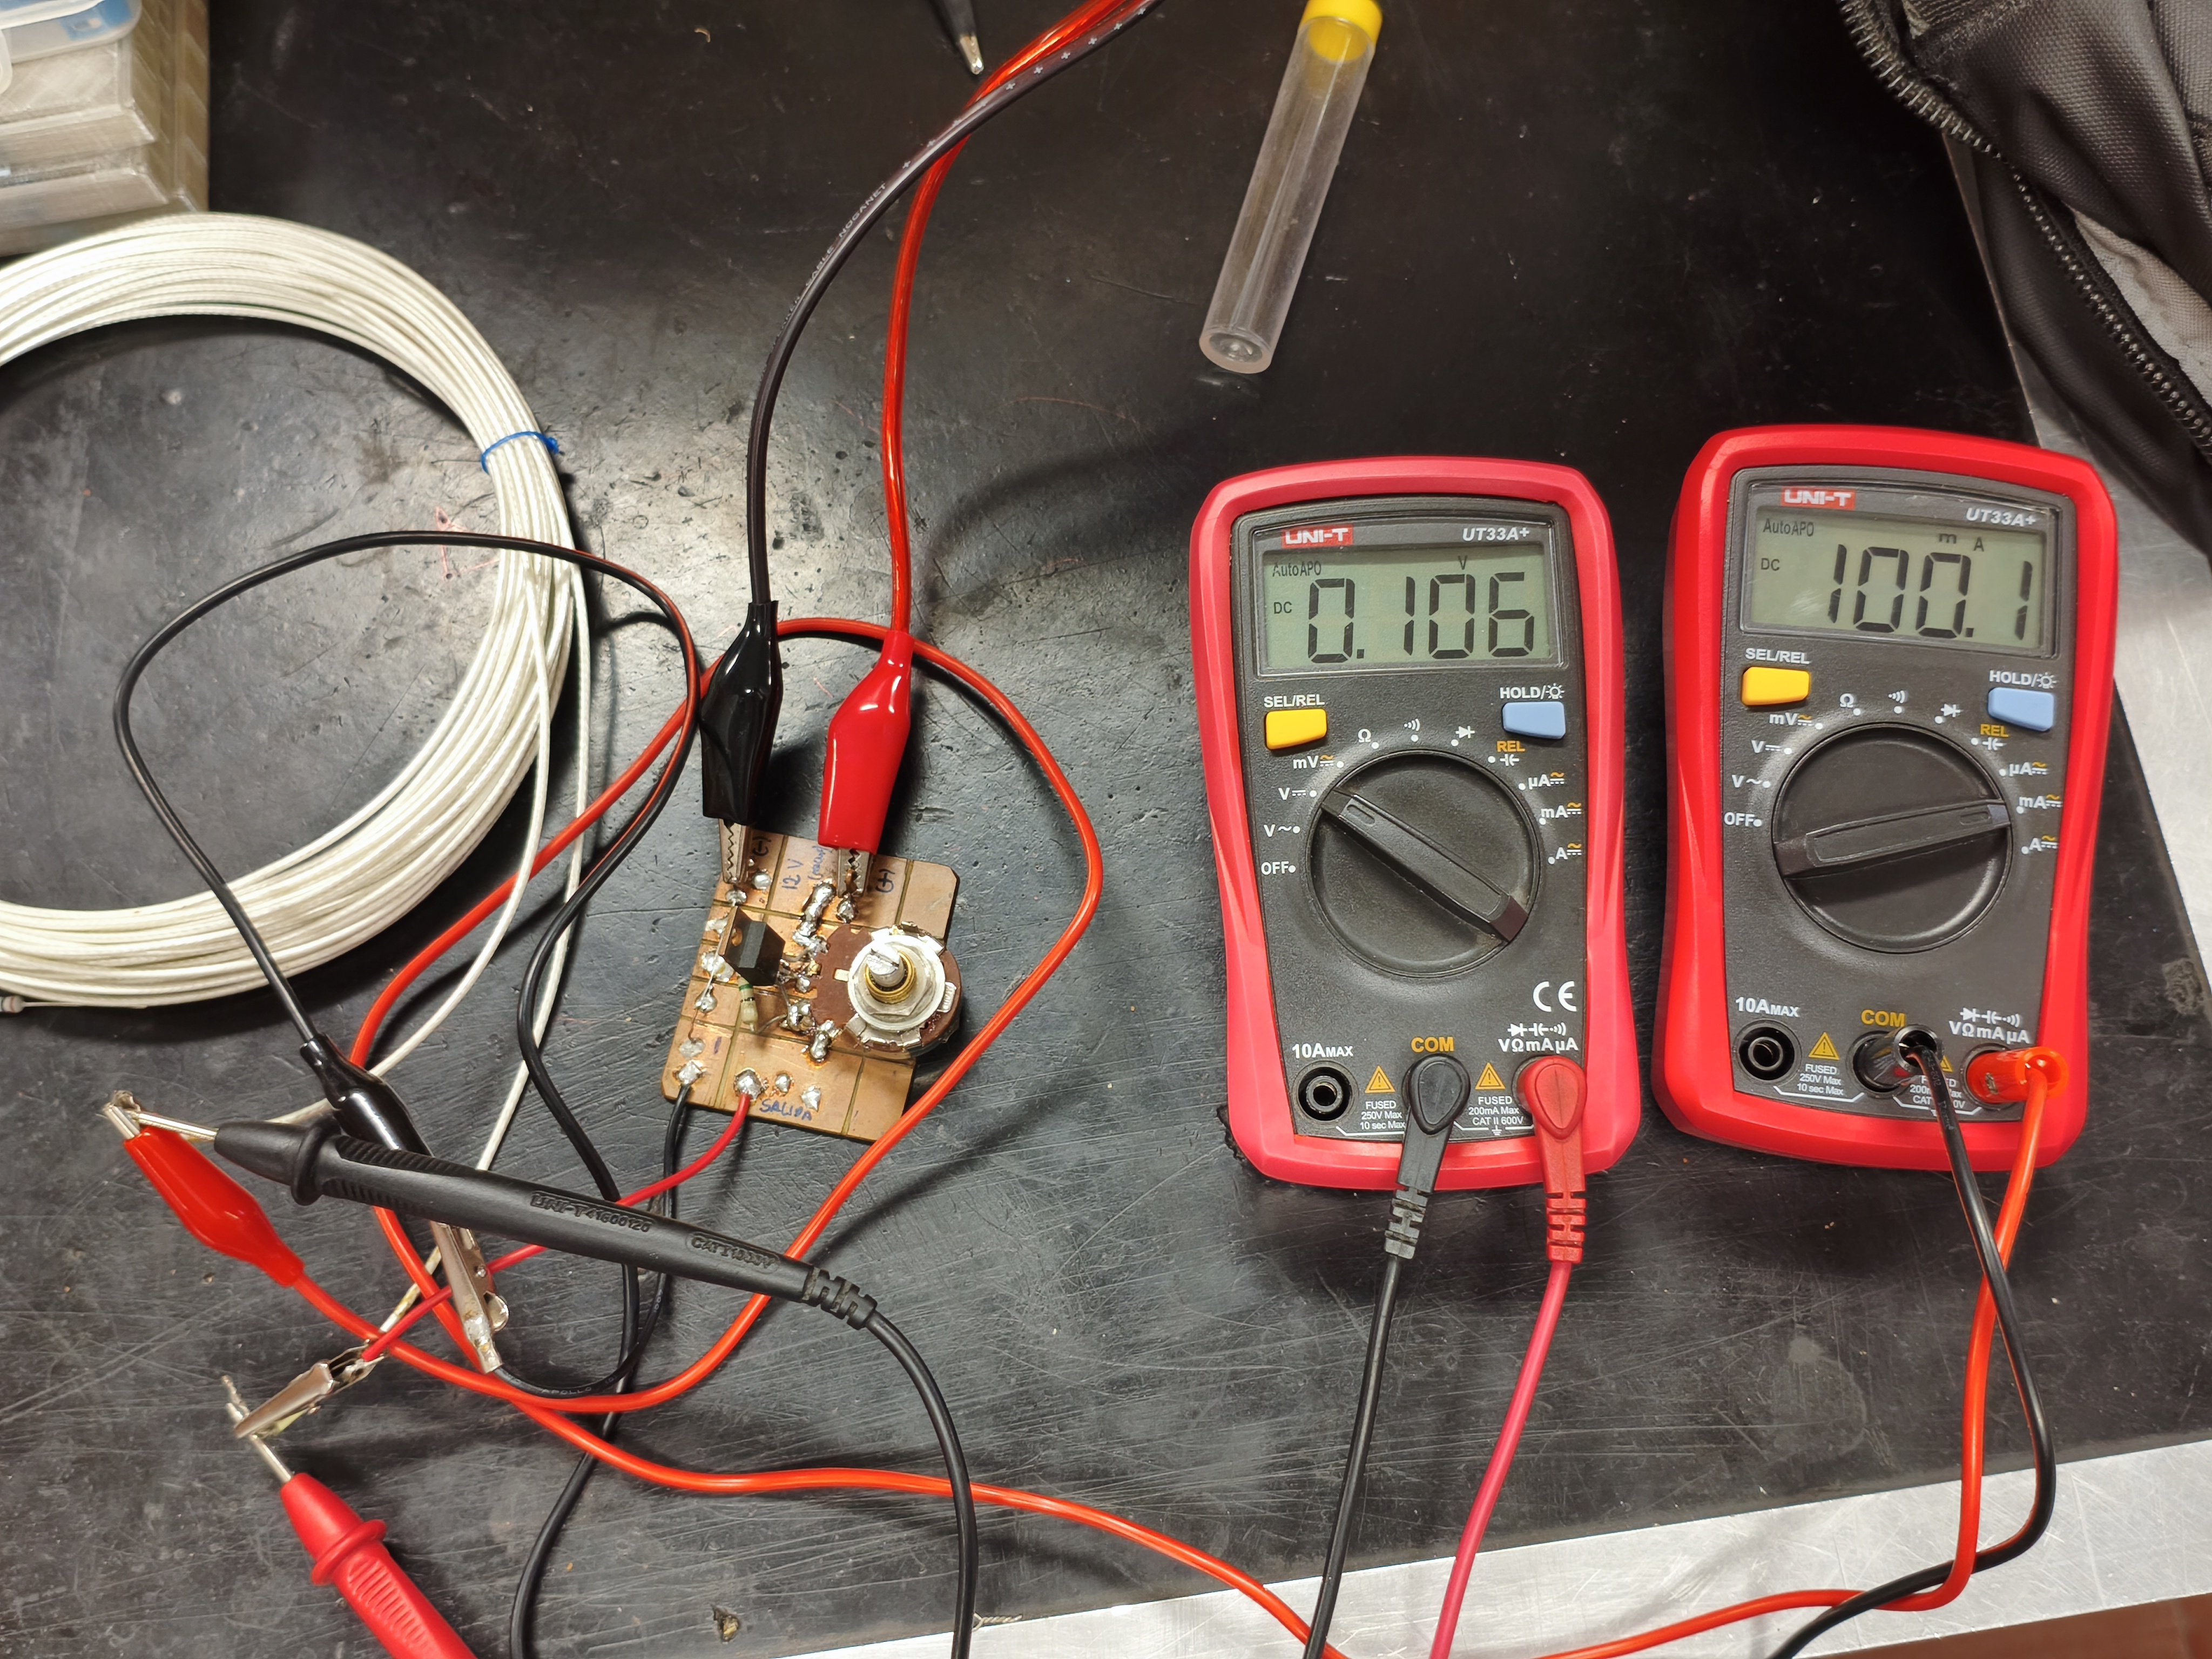
\includegraphics[width=\textwidth]{pictures/IMG_20261022_193557.jpg}
        \caption{Conexión de las 4 puntas y lectura simultánea en ambos multímetros UT33A+.}
    \end{subfigure}
    \caption{Montaje experimental de 4 terminales inyectando $100{,}1\mA$ y midiendo la caída de $106{,}0\mV$ en la probeta.}
    \label{fig:montaje_4term}
\end{figure}

\subsection{Cálculo de la Incertidumbre}
Para la determinación de la incertidumbre en la medición indirecta de $R = V/I$, los errores relativos máximos parciales se suman linealmente para obtener la cota superior del error relativo:
\begin{equation}
    \frac{\Delta R}{R} = \frac{\Delta V}{V} + \frac{\Delta I}{I}
    \label{eq:incertidumbre_prop}
\end{equation}

Tanto la caída de tensión como la corriente se registraron mediante multímetros digitales UNI-T UT33A+:
\begin{itemize}
    \item \textbf{Multímetro de Tensión (UT33A+):} Conectado en posición $V\text{=--}$ (autorango en escala de $2{,}000\V$), registrando $V = 0{,}106\V = 106{,}0\mV$ con una resolución de $0{,}001\V$ ($1\mV$). Según la hoja de especificaciones del fabricante, la exactitud para este rango es $\pm(0{,}5\percent + 2\text{ dígitos})$.
    \item \textbf{Multímetro de Corriente (UT33A+):} Conectado en posición $\mA\text{=--}$ (escala de $200{,}0\mA$), registrando $I = 100{,}1\mA$ con una resolución de $0{,}1\mA$. Según el manual del fabricante, la exactitud para este rango es $\pm(1{,}0\percent + 2\text{ dígitos})$.
\end{itemize}

Considerando a la especificación de exactitud del fabricante expresada en la forma:
\begin{equation}
    \pm\left(a\percent\,\text{rdg} + b\,\text{dig}\right)
    \label{eq:exactitud}
\end{equation}
la incertidumbre absoluta instrumental resulta:
\begin{equation}
    \Delta x = \pm\left(\frac{a\percent \cdot \text{lectura}}{100} + b \cdot \text{resolución}\right)
    \label{eq:calculo_incertidumbre}
\end{equation}

Aplicando los valores experimentales:
\begin{equation}
    \Delta V = \pm\left(\frac{0{,}5\percent \cdot 0{,}106\V}{100} + 2 \cdot 0{,}001\V\right) = \pm 0{,}00253\V = \pm 2{,}53\mV
    \label{eq:incertidumbre_tension}
\end{equation}

\begin{equation}
    \Delta I = \pm\left(\frac{1{,}0\percent \cdot 100{,}1\mA}{100} + 2 \cdot 0{,}1\mA\right) = \pm 1{,}201\mA
    \label{eq:incertidumbre_corriente}
\end{equation}

A partir de las incertidumbres absolutas, se obtienen las incertidumbres relativas:
\begin{equation}
    \frac{\Delta V}{V} = \frac{0{,}00253\V}{0{,}106\V} = 0{,}02387 \approx 2{,}39\percent
    \label{eq:incertidumbre_rel_tension}
\end{equation}

\begin{equation}
    \frac{\Delta I}{I} = \frac{1{,}201\mA}{100{,}1\mA} = 0{,}01200 \approx 1{,}20\percent
    \label{eq:incertidumbre_rel_corriente}
\end{equation}

Por lo tanto, la incertidumbre relativa total combinada (peor caso) de la resistencia calculada es:
\begin{equation}
    \frac{\Delta R}{R} = \frac{\Delta V}{V} + \frac{\Delta I}{I} = 0{,}02387 + 0{,}01200 = 0{,}03587 \approx 3{,}59\percent
    \label{eq:incertidumbre_resistencia}
\end{equation}

La incertidumbre absoluta de la resistencia resulta:
\begin{equation}
    \Delta R = \frac{\Delta R}{R} \cdot R = 0{,}03587 \cdot 1{,}05894\,\Omega \approx 0{,}038\,\Omega \approx 0{,}04\,\Omega
    \label{eq:incertidumbre_abs_r}
\end{equation}

\textit{Nota:} Si se evalúa la incertidumbre combinada mediante la raíz de la suma de cuadrados (RSS), se obtiene:
\begin{equation}
    \left(\frac{\Delta R}{R}\right)_{\text{RSS}} = \sqrt{\left(\frac{\Delta V}{V}\right)^2 + \left(\frac{\Delta I}{I}\right)^2} = \sqrt{(0{,}02387)^2 + (0{,}01200)^2} = 0{,}0267 \approx 2{,}67\percent
\end{equation}
lo que conduce a $\Delta R_{\text{RSS}} \approx 0{,}028\,\Omega$.

Todos los valores de incertidumbre calculados se resumen de forma comparativa en el cuadro \ref{tab:incertidumbres}.

\begin{table}[!ht]
    \centering
    \resizebox{\textwidth}{!}{
    \begin{tabular}{|c|c|c|c|c|}
        \hline
        Magnitud & Valor Medido & Incertidumbre Abs. ($\Delta x$) & Inc. Relativa $\left(\frac{\Delta x}{X}\right)$ &
        Inc. Rel. Porcentual $\left(\frac{\Delta x}{X} \cdot 100\right)$ \\ \hline
        $V$ & $106{,}0 \mV$ ($0{,}106 \V$) & $2{,}53 \mV$ ($0{,}00253 \V$) & 0,0239 & $2{,}39 \percent$ \\ \hline
        $I$ & $100{,}1 \mA$ & $1{,}201 \mA$ & 0,0120 & $1{,}20 \percent$ \\ \hline
        $R = V/I$ & $1{,}059 \ohm$ & $0{,}038 \ohm$ & 0,0359 & $3{,}59 \percent$ \\ \hline
    \end{tabular}}
    \caption{Desglose de valores de medición e incertidumbre por el método de 4 terminales.}
    \label{tab:incertidumbres}
\end{table}

\textbf{Resultado Final:} $R = (1{,}06 \pm 0{,}04)\,\ohm$ \quad (o con tres cifras decimales: $R = (1{,}059 \pm 0{,}038)\,\ohm$)

\section{Experimento 3: Resistencia de un Sistema de Puesta a Tierra}
\textbf{Fecha de la experiencia:} Jueves 27 de Marzo en el horario de clases.

Para medir la resistencia de la jabalina del "Laboratorio Central de Electrónica" (caja ubicada debajo del pizarrón), se
empleó el telurímetro UNI-T UT522 con un montaje de electrodos auxiliares sobre paños húmedos en el piso del pasillo
exterior, emulando una malla conductora. Se seleccionó inicialmente el rango de $400 \Omega$ y luego se bajó al de
$40 \Omega$ para obtener mayor resolución.

\begin{figure}[!ht]
    \centering
    \begin{subfigure}[t]{0.45\textwidth}
        \centering
        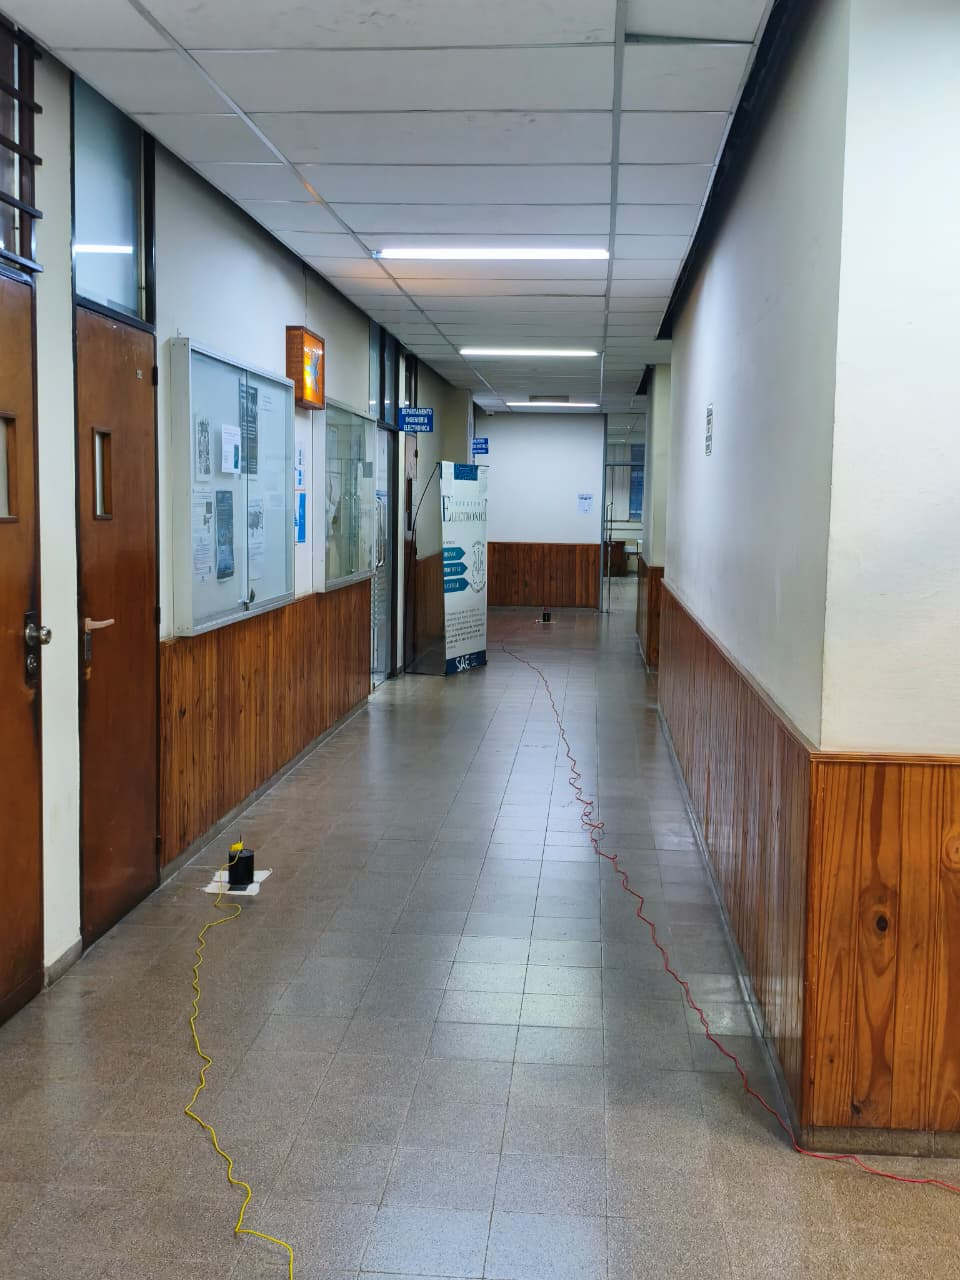
\includegraphics[width=\textwidth]{pictures/SetupjMedicionRJabalina_1.jpeg}
        \caption{Disposición de los electrodos auxiliares en el pasillo.}
    \end{subfigure}
    \hfill
    \begin{subfigure}[t]{0.45\textwidth}
        \centering
        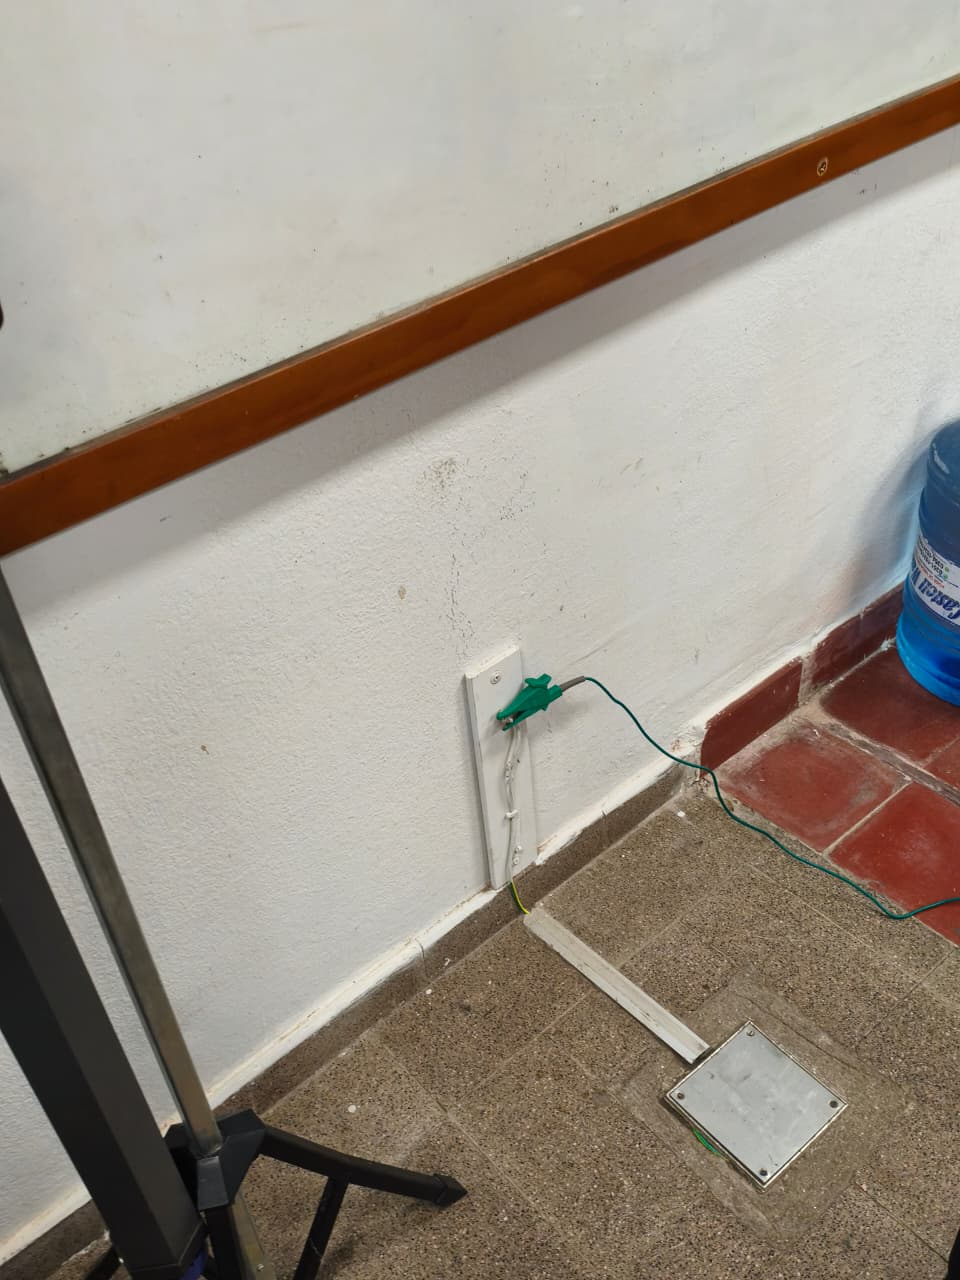
\includegraphics[width=\textwidth]{pictures/SetupjMedicionRJabalina_2.jpeg}
        \caption{Conexión a la bornera de puesta a tierra (jabalina).}
    \end{subfigure}
    \caption{Montaje para la medición de resistencia de tierra.}
    \label{fig:setup_jabalina}
\end{figure}

\begin{itemize}
    \item \textbf{Valor leído $R(Jabalina)$:} $0,79 \ohm$ (en escala de $40 \ohm$).
\end{itemize}

\begin{figure}[!ht]
    \centering
    \begin{subfigure}[t]{0.45\textwidth}
        \centering
        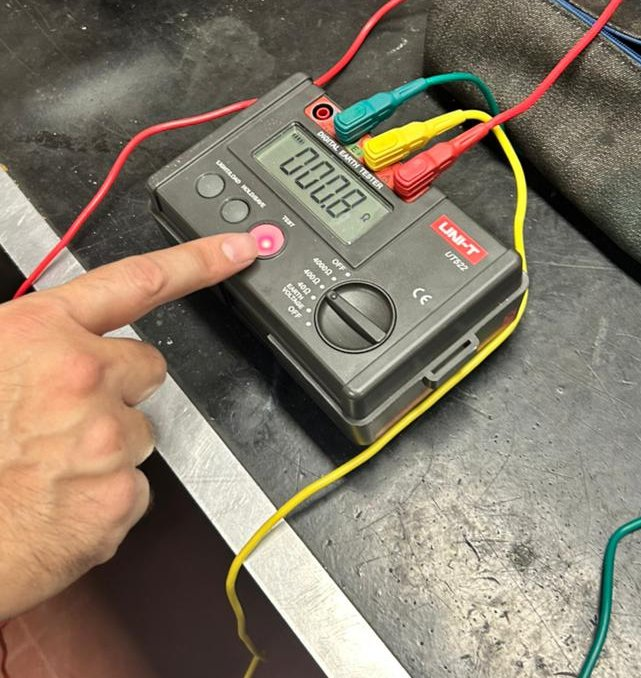
\includegraphics[width=\textwidth]{pictures/MedicionRjabalibna_escala_400ohm.jpeg}
        \caption{Lectura en escala de $400 \ohm$ ($0,8 \ohm$).}
    \end{subfigure}
    \hfill
    \begin{subfigure}[t]{0.45\textwidth}
        \centering
        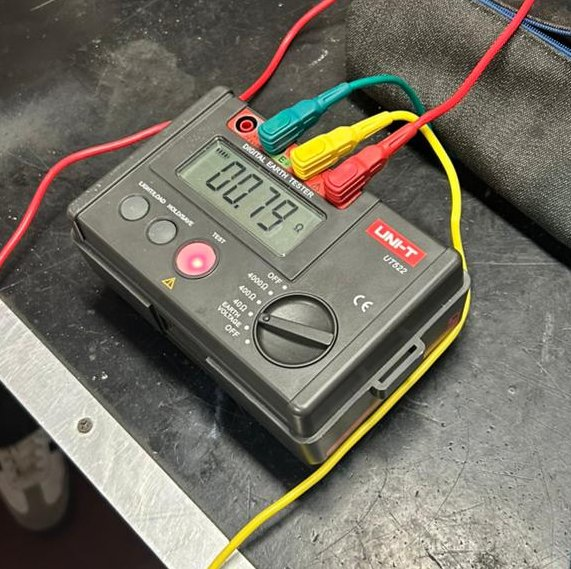
\includegraphics[width=\textwidth]{pictures/MedicionRjabalibna_escala_40ohm.jpeg}
        \caption{Lectura en escala de $40 \ohm$ ($0,79 \ohm$).}
    \end{subfigure}
    \caption{Comparación de lecturas según la escala seleccionada.}
    \label{fig:lecturas_jabalina}
\end{figure}

De acuerdo al manual del instrumento, las especificaciones son:
\begin{itemize}
    \item Rango $40 \ohm$: $\pm(2.0 \percent + 20)$
    \item Rangos $400 \ohm$ y $4000 \ohm$: $\pm(2.0 \percent + 3)$
\end{itemize}

Considerando la lectura obtenida en el rango de $40 \ohm$, la incertidumbre presente en la medición es:
\begin{equation}
    \Delta R = 0,79 \ohm \cdot 0,02 + 20 \cdot 0,01 \ohm = 0,0158 \ohm + 0,20 \ohm = 0,2158 \ohm \approx 0,22 \ohm
\end{equation}

\begin{itemize}
    \item \textbf{$R_j$ (con incertidumbre):} $(0,79 \pm 0,22) \ohm$
\end{itemize}
